\begin{section}{Preguntas}

A continuación pasamos a responder algunas de las preguntas enunciadas en el trabajo práctico.
\begin{itemize}
	\item ¿Depende la forma de la curva de la elección de la parametrización?
	
		Como vimos en los gráficos de la sección resultados, la elección de la parametrización está completamente ligada a la forma de la curva. Como ejemplo de esto podemos hacer referencia a los gráficos \ref{fig:5p}, \ref{fig:5p_r} y \ref{fig:5p_u}. Si bien todas las parametrizaciones comparten ciertos puntos (por ejemplo los mismos puntos de control), la forma en que aproximan a la curva es distinta.

	\item ¿Cambia la forma de la curva si en lugar de deformar la curva conservando la parametrización el programa la recalcula al mover el punto?

	Para poder responder esta pregunta deformamos la curva manteniendo la parametrización y recalculándola (el código implementa la primer opción). Graficamos los resultados, donde en cada uno de ellos se utilizó sólo una parametrización. La curva original es igual para los tres gráficos.
	Se presentan los mismos en el siguiente orden, utilizando la parametrización uniforme, la centrípeta y por último por longitud de cuerda.
	
	En las figuras visualizamos en color $rojo$ la curva original y los puntos de control. En $negro$ el punto seleccionado y en $rosa$ el punto en la curva más proximo a este.
	Vemos también en $azul$ la curva modificada manteniendo la parametrización y en $verde$ la curva deformada recalculándola.
	\begin{figure}[H]
		  \centering
			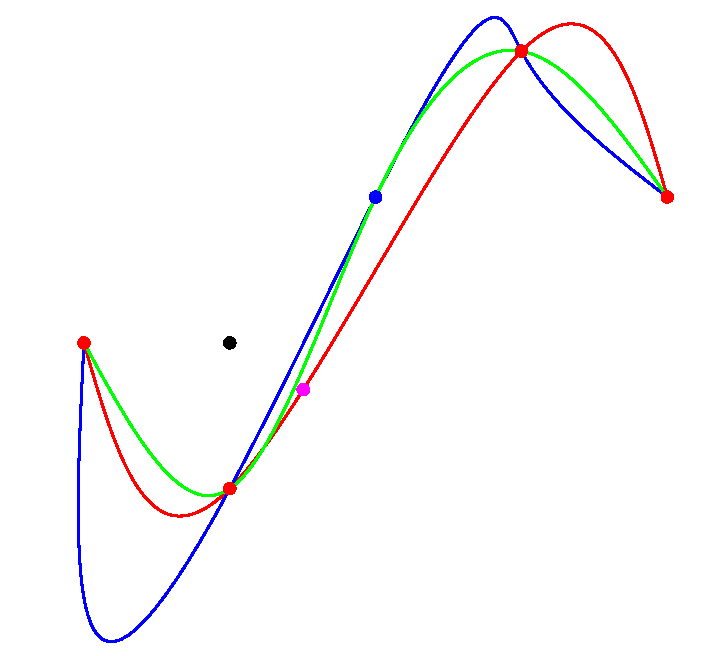
\includegraphics[width=7cm]{graficos/paramVSreparamUniform.pdf}
		  \caption{Cambio de parametrización (Uniforme)}
		  \label{fig:paramChangeUniform}
	\end{figure}
	
	\VSP
	
	\begin{figure}[H]
		  \centering
			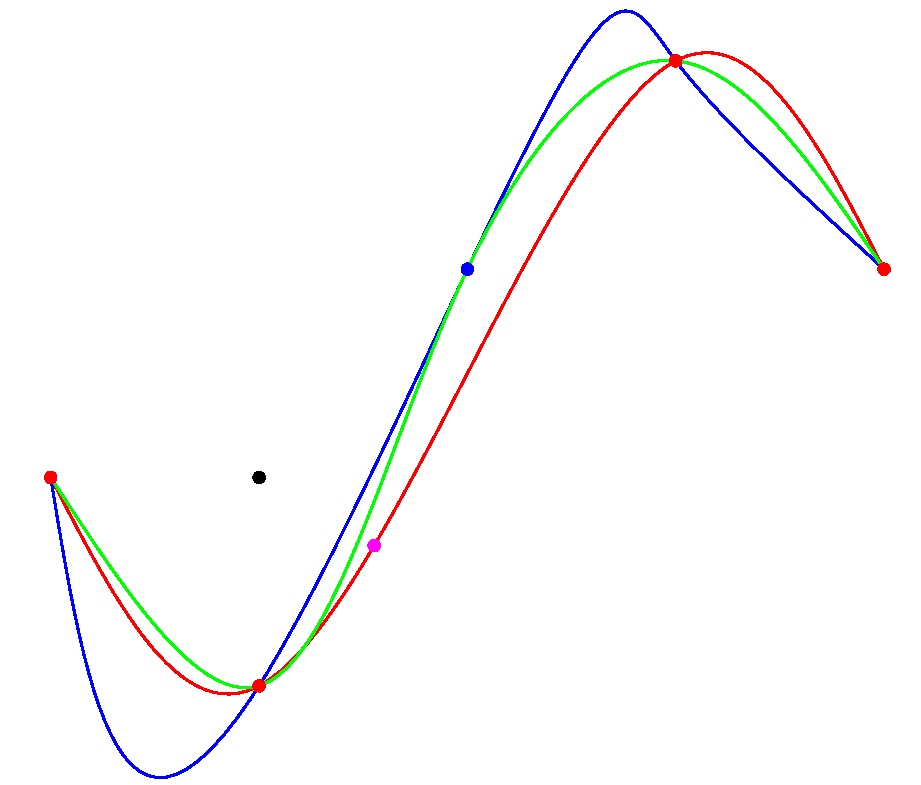
\includegraphics[width=7cm]{graficos/paramVSreparamCentripetal.pdf}
		  \caption{Cambio de parametrización (Centrípeta)}
		  \label{fig:paramChangeCentripetal}
	\end{figure}
	
	\VSP
	
	\begin{figure}[H]
		  \centering
			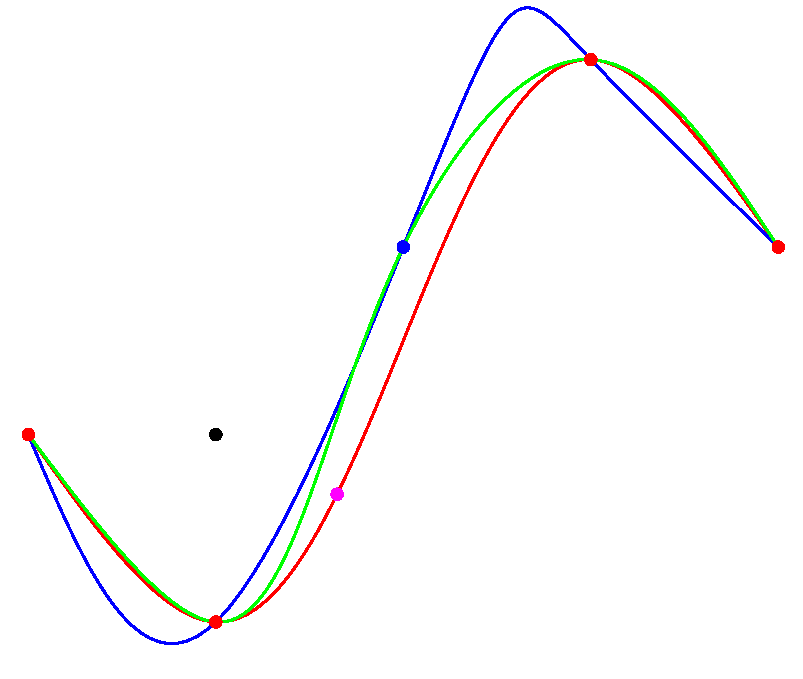
\includegraphics[width=7cm]{graficos/paramVSreparamChord.pdf}
		  \caption{Cambio de parametrización (Longitud de cuerda)}
		  \label{fig:paramChangeCHLength}
	\end{figure}
	
	\VSP
	
	Efectivamente la forma de la curva cambia al recalcular la parametrización respecto a no hacerlo. 
	
	Las curvas donde se recalcula la parametrización (curva $verde$) en las $tres$ figuras (usando cualquiera de las parametrizaciones) tienen una forma más similar a la curva original en los puntos alejados 
	al punto movido en contraste con la curva que mantiene la parametrización (curva $azul$). 
	%ya que esta cambia de manera proporcional a la distancia entre la posición del punto más próximo al elegido ($rosa$) y la posición final del mismo ($azul$).

	\item (Opcional) Luego de mover el punto seleccionado, ¿cambia toda la curva (control global) o sólamente una parte (control local)? ¿Qué consecuencias puede tener esto?
	
	Como ya vimos, cambia toda la curva, aunque el cambio es más abrupto en el punto perteneciente a la curva original, esta diferencia se va minimizando a medida que esta se aleja del punto seleccionado.
	
	Supongamos que tenemos un $set$ de datos que efectivamente pertenecen a una función y unos pocos datos anómalos, el resultado obtenido puede llegar a distar mucho del resultado que debería ser, ya que la curva completa se perturba por la existencia de alguno de esos puntos.
	
	Supongamos que estamos en un programa de diseño gráfico y dibujamos una curva, es decir queremos obtener una forma en particular, nos damos cuenta que si bien la forma es la correcta, no es justo lo que qremos, no nos va a bastar con mover un punto ya que se deformaría en su totalidad.


	\end{itemize}	
\end{section}
